\section{Background}

We discuss how embedded systems and peripherals interact, and the challenge of providing peripheral-aware worst case energy consumption bounds, motivating the need to utilize typestate for a type-based approach to this problem. 

\subsection{Embedded Systems Basics}

An embedded system combines a processor with peripherals in order to perform actions such as timing, sensing and communication. The processor runs the main application code, and sends commands to peripherals to perform actions through the peripheral's API. However, not all commands are always valid for a given peripheral. For example, attempting to request a sensor to perform a measurement while it is turned off would fail. Many peripherals are \textit{stateful}, meaning they have an internal state that determines what commands can be accepted and performed. This internal state also determines the amount of power each peripheral draws from the main board as well. Importantly, this internal state can change either as a result of an API call, or by the hardware as a part of the peripheral's operation. This internal state is frequently represented as a state machine \sai{probably cite chibi here?}, and a simplified version of what such a state machine looks like for a common peripheral known as an I2C bus is shown in \autoref{fig:i2c_diagram}.
\begin{figure} \centering
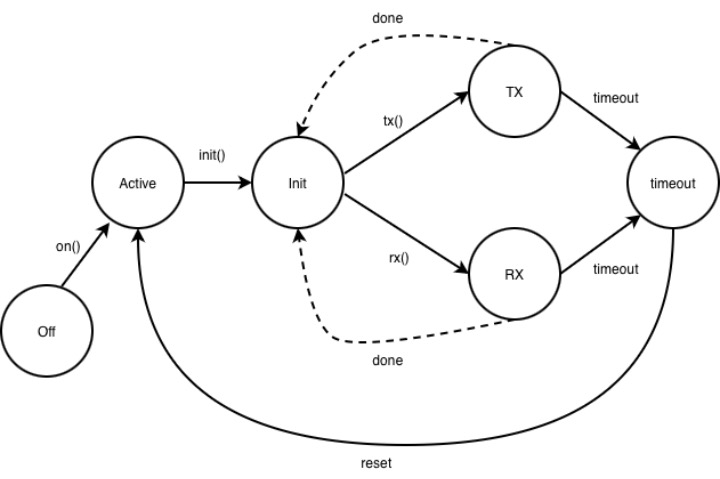
\includegraphics[width=0.5\linewidth]{diagram.jpeg} \caption{A simplified I2C bus state machine diagram}
\label{fig:i2c_diagram}
\end{figure}

Note that in the diagram, most edges are named with a specific function, this is because that function is what performs the state transition. However, the back-edges from the tx/rx state to the init state are represented with just "done." This is due to the hardware automatically transitioning back to the initalized state once it has finished performing it's action. Such transitions by hardware are common especially in low-power settings. In such settings, the processor will issue an initial command, and then continue to execute code until the hardware raises an interrupt that it has completed operation and transitioned back to a known state for the processor. When a peripheral is in a state where transitions are able to be performed by hardware, we call it \textit{unstable}, and we call states where transitions are only able to be performed by software \textit{stable}. Lastly, the processor clock affects the rate at which the processor executes cycles. This is important as certain peripherals such as the UART or I2C rely on the processor clock being a certain speed to operate correctly and efficiently. 

\subsection{Bounding Worst-Case Energy Consumption}

Worst-case energy consumption (WCEC) is the maximum energy a program can consume over its possible executions on a given platform. Broadly speaking, there are two main approaches to this problem. Measurement-based approaches estimate energy use by observing executions on hardware. The estimate depends on which inputs and device behaviors the measurements cover. Static analysis based approaches instead use a model of the program and hardware to bound the energy of possible executions. Recent work in this space has followed a similar high level structure: enumerate the possible runtime paths, and then translate into a formal constraint-satisfaction problem that can be solved when combined with hardware-specific information \cite{raffeck_et_al_OASIcs_WCET_2019_4,wegener_et_al_OASIcs_WCET_2023_9}.

For peripheral-aware analysis, the instructions executed by the processor only describe part of the system's activity. Peripherals consume energy when they perform work or change state, and they can continue to draw power while the processor executes unrelated code. The energy a peripheral consumes in a state depends on its power draw and how long it stays in that state. A clock change can affect the duration of processor work and, consequently, the time over which peripherals consume energy in the background. It can also affect the timing of peripherals that depend on the clock being changed. The primary approach that accounts for these factors is WoCA \cite{woca}, which uses peripheral state information combined with existing path enumeration techniques to provide a peripheral-aware energy consumption bound.

The actual bounds produced by prior work are largely derived from hardware-specific energy models, and provide concrete bounds in terms of the number of joules used. These can provide accurate bounds, but relies on such an energy model either being already present, or the user creating one for their own hardware. For Heliod, we instead opt to present costs in a symbolic manner. The major benefit of this symbolic cost calculation is that it enables relative reasoning of the energy consumption for the same program in a relatively hardware-agnostic manner. 

\subsection{Typestate and Type-Based Cost Analysis}

Typestate is a technique for encoding the runtime state of an object into the type system. This ensures that actions on a stateful object are only performed when the object is in the correct state. Abacus applies typestate to embedded peripherals by letting programmers describe device states and operations and generating Rust types that enforce those descriptions \cite{abacus}.

Type systems can also derive bounds on resource use. Automatic amortized resource analysis (AARA) associates potential with types and uses constraints generated during type inference to derive resource bounds \cite{Hoffmann_Jost_2022}. A cost semantics defines the resource consumed during execution and provides the basis for proving that a derived bound covers that cost.

Peripheral state gives a type-based energy analysis additional information about what to charge. Before a transition, the possible source states determine which transition costs the analysis must consider. While other code runs, the possible peripheral states determine which background costs it must include. This information also matters across function calls, since a function can receive a peripheral in different states at different call sites. Heliod uses typestate to carry this information into the analysis of both peripheral operations and their energy costs.